The approach we used consisted of 1) formulating a progress maximization along the trajectory while reaching the waypoints and 2) a curriculum training strategy to train a neural network policy using deep reinforcement learning. Furthermore, we initially reduced the problem setting to a 2D world with a different model, elektra VTOL3, before applying our findings in a 3D world and a quadrotor model. In the following, the policy architecture, reward function, learning strategy and training details that were used in order to train a minimum time flight policy is described. 

\subsection{Policy Architecture}
\label{subsec:policy_architeture}
The observations consist of two parts: the VTOL drone's state (body orientation, as well as the translational and rotational velocities) and the relative path to the next two waypoints. The observation vector is denoted as  $o(t) = \left[R_W(t), v_B(t), \omega_B(t), wp_B(t), nwp_B(t)\right],$ where $R_W(t)$, $v_B(t)$, $\omega_B(t)$, are the drone's rotation matrix, velocity, body rates and $wp_B(t)$, $nwp_B(t)$ are the relative path to the next two waypoints of the trajectory. The action vector produced by the policy $a(t) = \left[f_1,f_2,f_3,f_4\right]$ gives the PWM signals for each rotor individually. In Figure \ref{fig:actor} both observation and action space are illustrated, as well as the actor network architecture, which is a 2-layer multilayer perceptron (MLP). For more details on the network architecture see Section \ref{subsec:training_details}.

\begin{figure*}[h]
\centering
\begin{subfigure}[ht]{0.45\textwidth}
    \centering
    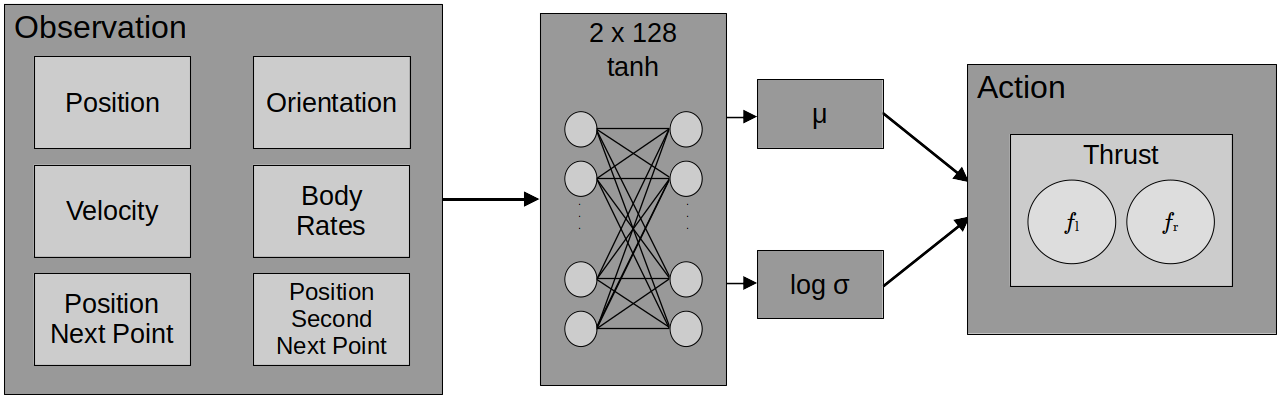
\includegraphics[width=1.0\textwidth]{images/2Dactor_short.png}
    \caption{Actor network for elektra VTOL3 controller in 2D world.}
    \label{fig:actor_2D}
\end{subfigure}
\hfill
\begin{subfigure}[h]{0.45\textwidth}
    \centering
    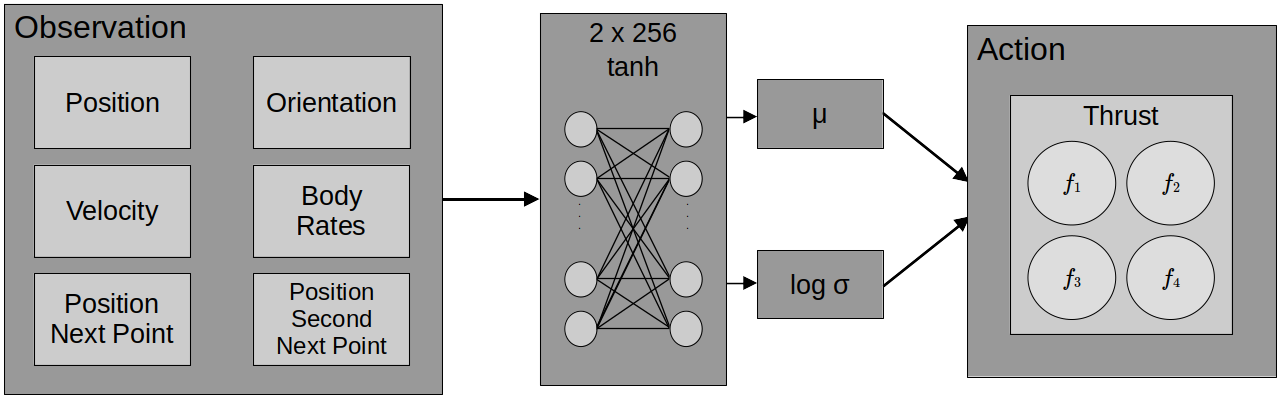
\includegraphics[width=1.0\textwidth]{images/3Dactor_short.png}
    \caption{Actor network for quadrotor controller in 3D world.}
    \label{fig:actor_2D}
\end{subfigure}
\caption{Illustration of the actor networks with the used observation and action spaces.}
\label{fig:actor}
\end{figure*}

\subsection{Reward Function}
\label{subsec:reward_fun}
The guiding trajectory is modeled as the connected lines between $n$ waypoints $g_1,...,g_n$. To calculate the progress at position $p$ we define the closest point on the trajectory as $\psi(p)$ and its corresponding line segment index as $l(p)$ as 
\begin{align}
\label{equ:progress_computation}
    l(p),\psi(p) &= \text{arg min}_{l(p),\psi(p)} \|p - \psi(p)\| \\
    \text{s.t. } & \psi(p) = g_{l(p)} + t (g_{l(p)+1} -  g_{l(p)}), \nonumber \\
     &t = \frac{(p - g_{l(p)}) \cdot (g_{l(p)+1} -  g_{l(p)})}{\|g_{l(p)+1} -  g_{l(p)}\|^2} , \nonumber \\
     &l(p) \in \{1,..,n-1\}, t \in [0,1]. \nonumber
\end{align}
The computation of the progress in time step $t$ is illustrated in Figure \ref{fig:trajectory}. 

\begin{figure}[b]
    \centering
    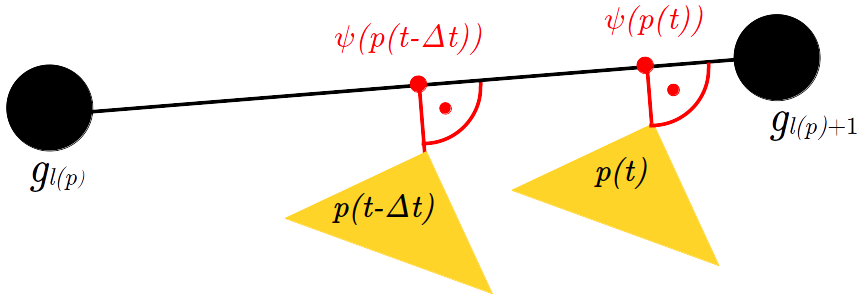
\includegraphics[width=0.3\textwidth]{images/trajectory.png}
    \caption{Illustration of trajectory with two waypoints. The nearest point $\psi(p)$ on trajectory from drone at position $p$ and its corresponding line segment index $l(p)$ is used to calculate the progress in each time step $\Delta t$ and the reached distance.}
    \label{fig:trajectory}
\end{figure}

The reward function consists of five main parts: encouraging progression along the trajectory in every time step, rewarding the overall reached distance along the trajectory, rewarding reached waypoints, penalizing high body rates $\omega$ and penalizing inactivity. This approach is leaned on the work of Penicka et al. \cite{Penicka_2022}.
The total reward function $r(t)$ at time $t$ is defined as 
\begin{align}
\label{equ:reward}
r(t) = k_p r_p(t) + k_s s(p(t)) + k_{wp} r_{wp} + k_\omega \|\omega\| - fall,
\end{align}
with the reached distance along the trajectory $s(p(t))$ and the progress reward at each time step $r_p(t)$ being defined as
\begin{align}
    &s(p) = \sum_{i=1}^{l(p) - 1} \| g_{i+1} - g_i \| + \|\psi(p) - g_{l(p)}\|, \\
    &r_p(t) = s(p(t))-s(p(t- \Delta t)).
\end{align}
The reached distance $s(p(t))$ is part of the reward function to counteract possible singularities due to sharp corners of the trajectory and the minimum distance projection. The reward $r_{wp}$ was payed, if the drone reached a waypoint within a distance $d_{wp}$ smaller than a tolerance $r_{tol}$ for the first time. The term $k_\omega \|\omega\|$ discourages high body rates. The penalty term $fall$ was only subtracted if the drone fell under $0$m due to inactivity. The contribution of each reward part is scaled by the hyperparameters $k_p$, $k_s$, $k_{wp}$ and $k_{\omega}$.

\subsection{Training Strategy} 
\label{subsec:training_strategy}
Optimizing the reward \eqref{equ:reward} directly could lead to suboptimal performance due to local minima and a higher risk of missing the waypoints in high speed flight. To overcome this we used a curriculum learning strategy. 

First, in an initial slow learning phase a slow and stable policy is trained that follows the trajectory closely and stays within a velocity range between $v_{min}$ and $v_{max}$. 
Second, a fast learning phase in which a racing policy was trained by encouraging velocities above a threshold $v_{min}$ while still reaching the waypoints. 

We achieve this by scaling the reward differently in the respective phase. The reward hyperparameters for progress $k_p$ and distance $k_s$ were scaled by a factor $s_m$ that encouraged translation velocities between $v_{min}$ and $v_{max}$. This scaling factor also motivates the drone to stay within a distance of $d_{max}$ to the trajectory. Note that $v_{min}$, $v_{max}$ and $d_{max}$ differ in the different phases. In the fast learning phase a dummy value for $v_{max}$ was inserted. The scaling factor $s_m$ is calculated as
\begin{align*}
     & s_m = s_{v} \cdot s_{gd}, \\
     & s_{v} = \min(1, 10^{v_{max}-||v||}) \cdot \min(1, 10^{||v||-v_{min}}), \\
     & s_{gd} = \min(1,e^{ - \|p - \psi(p) \| + d_{max}}).
\end{align*}

Furthermore, to ensure that the drone still reaches the waypoints even in high speed flight $k_p$ and $k_s$ were scaled down in the fast learning phase such that the term for reaching a point $k_{wp}r_{wp}$ was in comparison more rewarding. Ablating this scale down would lead to uncontrolled speedup and therefore to missing waypoints.  
Moreover, the parameter $k_{\omega}$ was reduced in the fast learning phase to allow for more rapid maneuvering. See Table \ref{table:parameters_learning_phase} for details on the parameters that were used for the respective phase. 


\begin{table*}[h]
        \centering
        \caption{Parameters of the algorithm.}
        \begin{tabular}{c @{\hspace{0.75\tabcolsep}} c |@{\hspace{0.75\tabcolsep}} c @{\hspace{0.75\tabcolsep}} c |@{\hspace{0.75\tabcolsep}} c @{\hspace{0.75\tabcolsep}} c |@{\hspace{0.75\tabcolsep}} c @{\hspace{0.75\tabcolsep}} c |@{\hspace{0.75\tabcolsep}} c @{\hspace{0.75\tabcolsep}} c |@{\hspace{0.75\tabcolsep}} c @{\hspace{0.75\tabcolsep}} c} 
             \hline
             \multicolumn{4}{c|@{\hspace{0.75\tabcolsep}}}{General parameters} &  \multicolumn{4}{c |@{\hspace{0.75\tabcolsep}}}{Slow learning phase} & \multicolumn{4}{c}{Fast learning phase} \\ [0.1ex] 
             \hline
             \hline 
             Variable & Value & Variable & Value & Variable & Value & Variable & Value & Variable & Value & Variable & Value  \\ [0.1ex] 
             \hline
             $\Delta t$ [s] & $0.025$ & $fall$ [-] & 1 & $v_{min}$ [m/s] & $1.0$ & $k_p$ [-] & $5.0 \cdot s_m$ & $v_{min}$ [m/s] & $4.0$ & $k_p$ [-] & $\frac{5.0 \cdot s_m}{\sum_{i=1}^{n-1} \|g_{i+1} -g_i\|}$\\ [0.2ex]
             $n$ [-] &  4  & $k_{wp}$ [-] & $50.0$ & $v_{max}$ [m/s] & $3.0$ & $k_\omega$ [-] & 0.01 & $v_{max}$ [m/s] & $50.0 $  & $k_\omega$ [-] & 0.001\\ [0.2ex]
             $r_{tol}$ [m] & 0.5 & $r_{wp}$ [-] & $\exp(\frac{d_{wp}}{r_{tol}})$ & $d_{max}$ [m] & 0.5 & $k_s$ [-] & $\frac{2v_{max}\Delta t \cdot s_m}{\sum_{i=1}^{n-1} \|g_{i+1} -g_i\|}$  & $d_{max}$ [m] & 1.0 & $k_s$ [-] & $\frac{2v_{max}\Delta t \cdot s_m }{\left(\sum_{i=1}^{n-1} \|g_{i+1} -g_i\|\right)^2}$ \\ [1.0ex]          
             \hline
        \end{tabular}
        \label{table:parameters_learning_phase}
    \end{table*}

\subsection{Training Details} 
\label{subsec:training_details}
We used an actor-critic algorithm as approximator. The applied optimization algorithm is Adam. The actor network produces actions learned via the Proximal Policy Optimization (PPO). Both actor and critic are multilayer perceptrons (MLP), see Table \ref{table:network} and Figure \ref{fig:actor} for details on their architectures. 

\begin{table*}[t]
\centering
\caption{Network architectures for elektra VTOL3 controller in 2D world and for quadrotor controller in 3D world.}
        
                \begin{tabular}{c|c|c|c|c|c|c|c|c} 
                 \hline 
                 Dimension & Network & Type & Input & Hidden Layer & Activation & Last Layer & Output & Output Size \\ [0.1ex] 
                 \hline
                 \hline
                 \multirow{3}*{2D} & \multirow{2}*{actor} & \multirow{2}*{MLP} & \multirow{2}*{observation} & \multirow{2}*{2x128} & \multirow{2}*{tanh} & 1x128 & action mean & 2 \\ [0.1ex]
                                   &                        &                    &                            &                      &                     & 1x128 & action variance & 2 \\ [0.1ex]
                 \cline{2-9}
                  & critic & MLP & observation & 2x128 & tanh & 1x128 & value & 1 \\ [0.1ex] 
                 \hline 
                 \multirow{3}*{3D} &\multirow{2}*{actor} & \multirow{2}*{MLP} & \multirow{2}*{observation} & \multirow{2}*{2x256} & \multirow{2}*{tanh} & 1x256 & action mean & 4 \\ [0.1ex]
                                   &                     &                    &                            &                      &                     & 1x256 & action variance & 4 \\ [0.1ex]
                 \cline{2-9}
                  & critic & MLP & observation & 2x256 & tanh & 1x128 & value & 1 \\ [0.1ex] 
                 \hline
                 \end{tabular}
\label{table:network}
\end{table*}

The policy was trained while utilizing 8 parallel agents. This increases the speed of collecting data and diversifies the experienced states and observations. For training we used the Julia environment Flyonic \cite{flyonic} that provides simulated models with the appropriate dynamics of elektra VTOL3 and a quadrotor.  

The training trajectories consisted of $n$ waypoints which were generated as follows: 
\begin{align}
\label{equ:trajectory_generation}
    & wp_1 = (0,0,0)^T, \text{  }  wp_i = wp_{i-1} + z_i \text{ for } i = 2,...,n 
\end{align}
where $z_i$ was sampled from the multivariate uniform distribution $\mathcal{U}_3$ on $[-7,7]\times 0 \times [1.5,7] \subseteq \mathbb{R}^3$ for the 2D world setting and  $[-3,3]\times [-3,3] \times [0.5,3] \subseteq \mathbb{R}^3$ for the 3D world setting. The distance ranges were decreased in the 3D setting since the quadrotor is significantly smaller than the elektra model.